\section{Zpětná západka}

Zpětnou západkou pohybuje motor pomocí magnetu. Pro zajištění vodě\-o\-dol\-nos\-ti je motor od západky oddělen stěnou, což je také jeden z~důvodů použití magne\-tic\-ké\-ho spojení.

\begin{figure}[h]
    \centering
    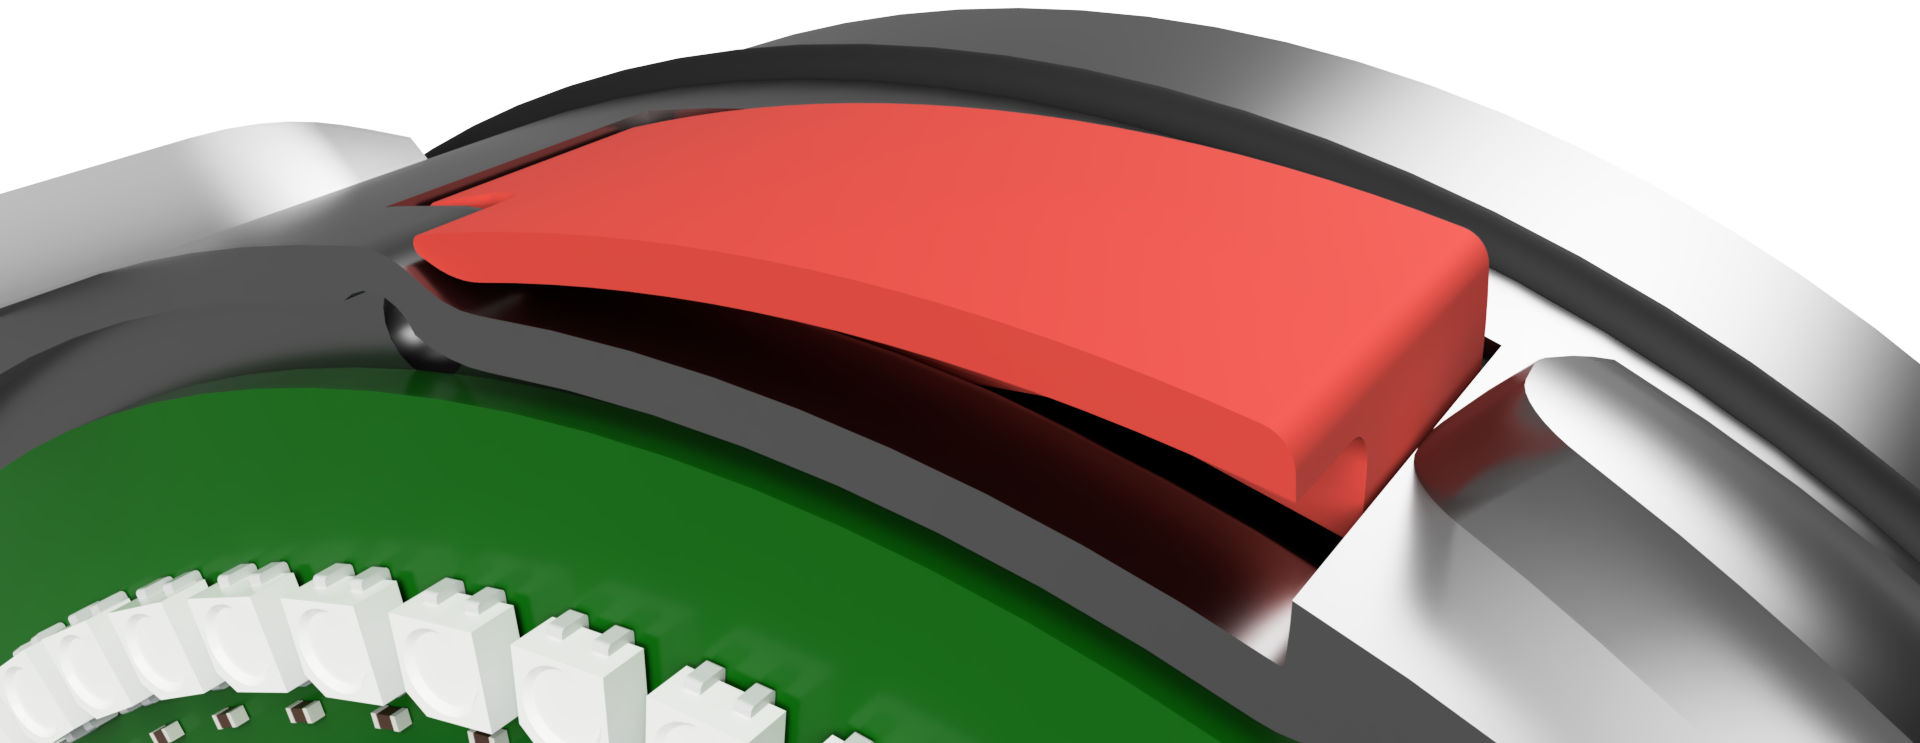
\includegraphics[width=\textwidth]{kapitoly/obrazky/E4/zapadka/render.png}
    \caption{Render západky}

    \label{fig:E4-zapadka}
\end{figure}

\paragraph{Sklon čela}
\addcontentsline{toc}{paragraph}{Sklon čela}

Aby při zamčení západka doléhala na otvor trezoru a zároveň neměla příliš velkou vůli, je potřebné správně navrhnout tvar západky.
Jednou z možností je navrhnout čelní plochu\footnote{Plocha, která je při zamčení v kontaktu se dveřním otvorem.} jako část válcové plochy. 
Sice teoreticky není problém na FDM tiskárně\footnote{typ 3D tiskárny tisknoucí z tiskové struny} vytisknout západku s takovou plochou čela,  %todo nechápu <- lepší?
a na laseru vypálit vhodný protikus\footnote{Stejná plocha totiž musí být i v otvoru do kterého se dveře umístí.},
ale výsledná plocha je hlavně u tisku nevzhledná a je třeba jí obrousit do požadovaného vzhledu. Obrousit válcovou plochu je však náročnější než plochu rovnou, zvlášť v otvoru trezoru, 
a je tedy pro mě výhodnější navrhnout tuto plochu jako rovinu a jen ji správně sklonit. Špatně navržený sklon by se projevil buď přílišnou vůlí, 
což by znamenalo, že by se dveře v trezoru viklaly a nebo by západka nebyla samosvorná, což by se projevilo možností trezor otevřít vetší silou 
i bez jeho odemčení.

\begin{figure}[htbp]
    \centering
    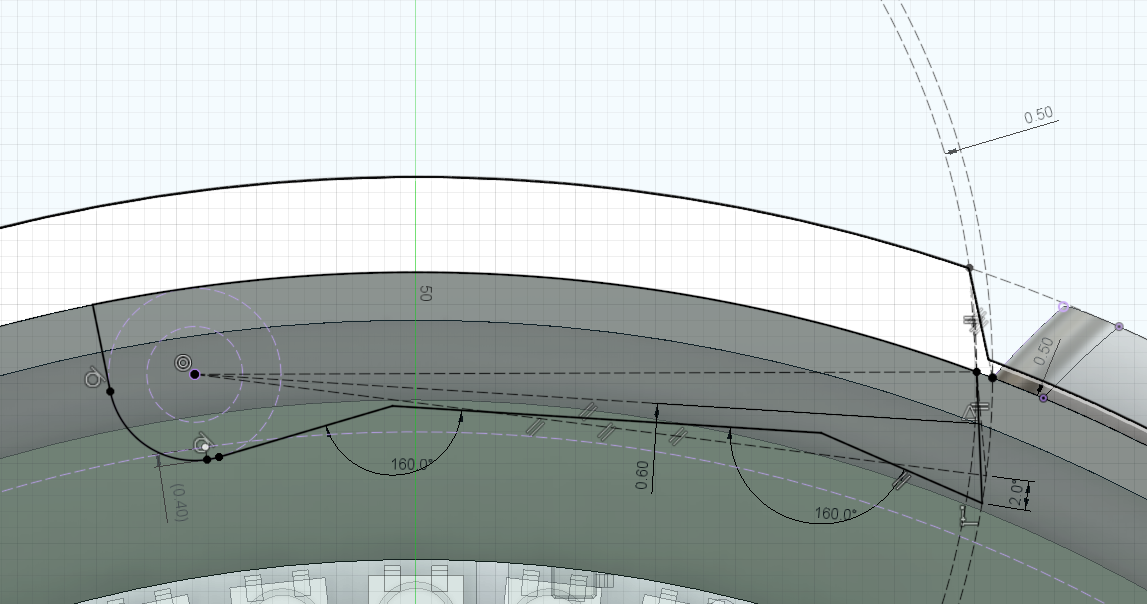
\includegraphics[width=\textwidth]{kapitoly/obrazky/E4/zapadka/uhel_cela.png}
    \caption{Geometrie západky}
    \label{fig:E4-uhel_cela_zapadky}
\end{figure}


\paragraph{Západka v průběhu vývoje}
\addcontentsline{toc}{paragraph}{západka v průběhu vývoje}

Západka se ve vývoji pochopitelně objevila společně s bajonetem, ale v první verzi byla jen částí těla dveří a teprve v~dalších verzích se stala
samostatnou součástkou. První tělo využívající bajonet jsem tiskl na FDM tiskárně z plastu PLA a západka byla jen jeho pružnou částí. Toto řešení sice 
z počátku fungovalo a mělo výhodu jednoduší výroby, ale PLA po několika měsících začalo ztrácet pružnost a západka se už nepohybovala v celém rozsahu.
Toto jsem z počátku chtěl řešit samostatnou západkou ve spojení s tažnou pružinou. Pružiny však nebyla třeba a naprosto stačí magnet na motoru a v západce.
Západka proto zůstala v teto podobě a~jen se přidala mechanická přepážka kvůli voděodolnosti. 

Západka je také v neposlední řadě navržena tak, aby odolala pokusu o vylomení za působení kroutícího momentu o velikosti až 5000 N$\cdot$mm, výsledky simulace najdete 
na obrázku \obr{fig:E4-simulace_zapadky}.
